\chapter{Systèmes de Gestion de Flux de Données}
Nous avons présenté dans le chapitre précédent les grands concepts de la gestion de flux de données. Celle-ci permet de répondre de manière intégré à l'interrogation continue sur des données dynamiques. Dans ce chapitre, nous allons donc explorer ce domaine d'un point de vue plus technique afin d'analyser les points clés manquants dans cette approche.

Afin de rendre les SGFD viables dans notre contexte. Après la présentation de l'approche, nous avons noté plusieurs faiblesses. Notre analyse portera donc particulièrement son attention sur les points clés suivants : 
\begin{itemize}
	\item[\textbf{Le langage}] : L'expressivité des langages manipulants les flux de données est bien plus complexe que le simple modèle relationnel. Le fait d'écrire des requêtes dont l'exécution ne s'arrête pas fait qu'il est nécessaire de prendre en compte l'évolution de son exécution. Afin qu'il soit possible d'exprimer les requêtes de façon claire, il est nécessaire d'avoir un langage et un modèle sous-jacent sans ambiguïté.
	\item[\textbf{Modes d'interrogations}] : Les SGFD sont capable uniquement d'exécuter des requêtes continues par nature. Toutefois, dans notre cadre, il est important d'être capable d'exprimer des requêtes instantanées ou mixtes. 
	\item[\textbf{Le support persistent}] : Dans le chapitre précédent, nous avons vu que le support de base de données permettait des analyses plus poussées. En effet, un flux est une entité transitoire, la durée de vie des données est par définition limité dans le temps. Or pour permettre des besoins d'analyse plus évoluées, il faut considérer le flux comme une entité complete. La capacité à archiver ces flux et à pouvoir l'interroger (de manière instantanée ou continue) sera primordial.
	\item[\textbf{Optimisation}] : Afin de s'adapter à tout type de systèmes, y compris à grande échelle. Il est nécessaire que l'exécution des requêtes soit efficace. En effet, cet aspect a des impacts prononcés au niveau de l'architecture ainsi que sur les algorithmes d'exécution des opérateurs.
\end{itemize}

\TODO{plan}
\section{Formalisations théoriques}\label{sec:rw:sgfd:modeles}
De nombreuses propositions ont été faites pour construire un modèle sur les flux en tentant de réutiliser les connaissances développées sur les systèmes de gestion de base de données relationnels depuis 40 ans.

Observer l'évolution des modèles au fur et à mesure des années permet en effet de cerner les problématiques théoriques liées à la gestion de flux. En~\ref{sec:rw:sgfd:modeles:early}, nous présentons les premiers modèles. En~\ref{sec:rw:sgfd:modeles:stream}, nous présentons la sémantique abstraite mélangeant flux et relations. Puis, nous présentons en~\ref{sec:rw:sgfd:modeles:batch} les initiatives de clarification et reformalisation des modèles existants.

\subsection{La genèse de la gestion de flux}\label{sec:rw:sgfd:modeles:early}
L'idée de créer des requêtes continues a été présentée en 1992 dans le système Tapestry~\cite{Terry:tapestry}. Dans ce système une requête continue est avant tout une requête instantanée exécutée périodiquement. Ces requêtes s'appliquent sur un ensemble de données sans suppression ou mise à jour (\textit{append-only}). Le résultat est représenté par le flux des nouvelles données calculées de manière incrémentale. Pour cela, les relations sont considérées comme des variables et elles deviennent dépendantes du temps.

En 1995, les flux de données ont été explorés tout d'abord par le modèle séquentiel $\mathcal{SEQ}$~\cite{Seshadri:seq}. Dans ce modèle, une \enquote{\it séquence} est un ensemble d'enregistrements (n-uplets relationnels) avec un ordre positionnel. Dans le modèle relationnel originel~\cite{Codd:model}, ceci n'est pas autorisé, car l'ordre des n-uplets est dit \enquote{\it irrelevant}. La définition des opérateurs relationnels utilise cette liberté d'ordre pour être consistante et obtenir des propriétés intéressantes (voir chapitre~\ref{chap:contrib:astral}). Le formalisme de $\mathcal{SEQ}$ montre qu'il est toujours possible d'exploiter les opérateurs algébriques relationnels classiques et d'en créer de nouveau comme les premières notions de regroupements de n-uplets appelés\textit{collapse}\footnote{Cette primitive représente ce qui est devenu l'opérateur de fenêtrage depuis}. Ce formalisme a été fondateur pour plusieurs des travaux futurs qui s'inspirent explicitement de ce modèle~\cite{Gurgen:sstreamware,Babcock:issues}.

Par la suite, les premières opérations sur les flux en tant que telles ont pu apparaître avec le système Chronicle~\cite{Jagadish:chronicle}. Toutefois, les flux étaient considérés soit comme un ensemble de données historiques, soit comme une donnée constamment mise à jour (fenêtres complètes, ou instantanées). La notion de fenêtre a été présentée pour la première fois dans Tribeca~\cite{Sullivan:tribeca,Sullivan:tribeca2}. Sa spécification est basée sur sa taille positionnelle (nombre de données) ou temporelle (durée). Toutefois, ce système ne peut gérer qu'un seul flux à la fois. La notion de fenêtre est désormais intégrée à SQL:1999~\cite{Melton:sql1999} ainsi que dans SQL:2003~\cite{Eisenberg:sql2003} pour des opérations OLAP.

Les requêtes continues ont été aussi développées pour interroger les bases de données dont le contenu est régulièrement mis à jour. À la fin des années 90, les bases de données contenant des pages et flux web dynamiques ont connu de graves problèmes de performances lors de l'analyse de flux d'événements. Ceci a été l'objet de projets tels que OpenCQ~\cite{Liu:opencq} et NiagaraCQ~\cite{Chen:niagaracq} qui permet de faire des opérations de jointures.

Le début des années 2000 a marqué l'avènement des systèmes de gestion de flux de données à part entière. L'arrivée d'applications réseaux~\cite{Cranor:gigascope} et capteurs~\cite{Madden:tag,Yao:cougar} a permis le développement des SGFD, car les besoins en performances et en puissance d'expression devenaient de plus en plus grand. À quelques mois d'intervalles, les premiers SGFD ont fait leur apparition : TelegraphCQ~\cite{Chandrasekaran:telegraphcq}, STREAM~\cite{Widom:queries} et Aurora~\cite{Carney:monitoring}. Ce dernier apporte de plus : SQuAl~\cite{Abadi:aurora}, la première algèbre complète sur les flux de données. Un flux est considéré comme un ensemble de n-uplets strictement ordonnés avec un schéma prédéfinit $(\textbf{TS}, A_1,\dots, A_n)$, où $\textbf{TS}$ correspond au \textit{timestamp}. L'algèbre décrit le comportement d'opérateurs simples comme la sélection (\textit{Filter}), la projection-évaluation (\textit{Map}) et l'union (\textit{Union}). Mais aussi d'opérateurs complexes (i.e. utilisant une fenêtre) tels que le tri à la volée (\textit{BSort}), l'agrégat (\textit{Aggregate}), la jointure sur bande (\textit{Join}) et un opérateur de synchronisation de \textit{timestamp} (\textit{Resample}). Il est important de noter que ces opérateurs complexes s'utilisent grâce à des fenêtres définies à l'avance.

TelegraphCQ~\cite{Chandrasekaran:telegraphcq} quant à lui propose un langage de requête beaucoup plus axé sur le relationnel avec notamment une définition de fenêtre générique. En effet, ces dernières étaient décrites par une séquence de type \textit{boucle for}.
\begin{center}
\begin{minipage}[c]{0.75\textwidth}
\begin{verbatim}
for(t=initial_value; continue_condition(t); change(t)) {
    WindowIs(StreamA, left_end(t), right_end(t));
    WindowIs(StreamB, left_end(t), right_end(t)); ?
}
\end{verbatim}
\end{minipage}
\end{center}

Cependant, depuis le début des requêtes continues, la spécification des opérateurs était avant tout dirigée par l'implémentation. Cela a amené à des limitations d'expressivité (voire des divergences d'interprétation) qui ont été traitées dans le SGFD générique STREAM.

\subsection{La sémantique abstraite à deux concepts}\label{sec:rw:sgfd:modeles:stream}
Le système STREAM~\cite{Widom:queries, Arasu:stream} se démarque des autres systèmes de son époque pour avoir décrit une sémantique abstraite qui distingue les concepts de flux et de relation~\cite{Arasu:semantic} :
\begin{itemize}
 \item[\textbf{Un flux}] est un ensemble potentiellement infini de n-uplets conformes à un schéma commun possédant un \textit{timestamp}.
 \item[\textbf{Une relation}] est une fonction qui associe le temps à un ensemble fini de n-uplets conformes à un schéma commun.
\end{itemize}
Le point crucial de cette approche est que les opérateurs permettent de passer d'un concept à l'autre (voir figure~\ref{fig:rw:sgfd:streamrelation}). Les opérateurs capables de traiter des relations pour en fournir une nouvelle sont les opérateurs relationnels (sélection, projection, jointure). Ceux-ci sont une adaptation de l'algèbre relationnelle. Les opérateurs transformant un flux en relation sont les opérateurs de fenêtres. Les opérateurs transformant les flux en relations sont des \textit{streamers}.
\begin{figure}[ht]
    \centering
    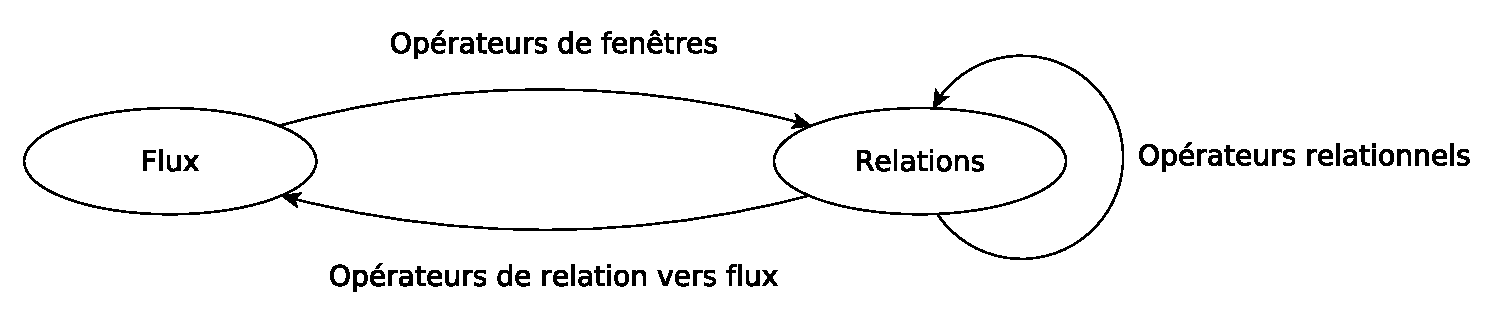
\includegraphics[width=0.75\textwidth]{rw-sgfd-streamrelation}
    \caption{Transformations appliquées dans la sémantique abstraite de STREAM}\label{fig:rw:sgfd:streamrelation}
\end{figure}

Afin de mieux illustrer la sémantique abstraite utilisée, nous allons détailler un exemple plus concret.
\begin{example}
Soit $S$ un flux de capteurs $(\mathrm{temperature}, \textbf{T})$ avec \textbf{T} pour \textit{timestamp} et temperature pour sa mesure. Nous souhaitons faire un agrégat sur 5 min. La composition des opérateurs est la suivante :
\begin{itemize}
\item D'abord un opérateur de fenêtrage $[5min]$ est appliqué. Il transforme le flux en la relation \enquote{\it groupement des 5 dernières minutes} qui évolue au cours du temps.
\item Ensuite un opérateur d'agrégation\footnote{notation simplifiée de l'opérateur d'agrégation sans groupement dont le résultat est une relation avec un seul attribut \textit{avg}} $\mathcal G_{avg(temp)}$ produit une relation avec un seul n-uplet.
\item Enfin, un opérateur de \textup{streaming} est appliqué. Celui-ci peut avoir plusieurs sémantiques. Prenons le plus simple $ISTREAM$ qui permet de créer un flux à partir des insertions dans la relation. Une mise à jour est considérée comme une suppression suivie d'une insertion.
\end{itemize}
La requête finale est : $$ISTREAM(\mathcal G_{avg(temp)}(S[5min]))$$
\end{example}

Le point clé et novateur de cette approche est que les opérateurs de flux vers flux \textbf{n'existent pas}. En particulier, la jointure de deux flux n'existe pas. Seule la jointure de relations est possible et la création des relations se fait à partir de fenêtres sur des flux. Les auteurs ont justifié cette approche, car l'écriture de requête est plus intuitive et que cela permet de généraliser l'utilisation des vues matérialisées dans le traitement des flux (introduit auparavant dans Chronicle~\cite{Jagadish:chronicle}). La spécification de cette sémantique a permis par la suite de décrire le langage associé CQL~\cite{Arasu:cql} (\textit{Continuous Query Language}) dérivé du \textit{SQL} qui est désormais utilisé dans de nombreux produits académiques et commerciaux~\cite{Witkowski:oraclecq,url:sqlstream}.

\begin{example}
La requête \textit{CQL} de l'exemple précédent a la forme suivante : 
\begin{center}
\it ISTREAM(SELECT AVG(temp) as avg FROM S [RANGE 5min])
\end{center}
\end{example}

La sémantique formelle du langage CQL est présentée dans la thèse d'Arvind Arasu~\cite{Arasu:queries}. L'algèbre \textit{ACO} (\textit{Algebra of Continuous Operators}) y est décrite. Les définitions élémentaires sont les suivantes :
\begin{itemize}
 \item[\textbf{Instant} ($\tau$)] : élément de l'ensemble $\mathcal T$, discret et ordonné\footnote{Il est en réalité définit comme un ensemble satisfaisant les axiomes de Peano. En particulier la présence d'un unique successeur. L'instant de départ de l'exécution est le plus petit instant observé $0$.} et représenté par $\N$.
 \item[\textbf{Relation}] : Fonction associant un instant à un multiensemble de n-uplets avec un schéma commun.
 \item[\textbf{Flux}] : Multi-ensemble d'éléments $\left<s,\tau\right>$ où $s$ est un n-uplet respectant un schéma commun et $\tau \in \mathcal T$ son \textit{timestamp}. Pour un $\tau$ donné, il existe un nombre fini (mais non borné) d'éléments.
\end{itemize}
Des opérateurs sont définis sur ces éléments. Les opérateurs relationnels sont simples car pour une \textit{relation} $R$, et un instant $\tau$ : la \textit{relation instantanée} $R(\tau)$ est une relation au sens SGBD\footnote{D'un point de vue strict, les multi-ensembles sont utilisés dans les SGBD mais ne font pas parti du modèle relationnel.}. Les opérateurs classiques peuvent être utilisés. Les équivalences suivantes sont vérifiées : $\forall \tau\in\mathcal T,$ 
\begin{eqnarray*}
    (\sigma_c R)(\tau) & = & \sigma_c(R(\tau))\\
    (R_1 \Join R_2)(\tau) & = & R_1(\tau) \Join R_2(\tau)
\end{eqnarray*}

Les opérateurs les plus importants sont ceux de classe $S2R$ (\textit{stream-to-relation}) et $R2S$ (\textit{relation-to-stream}). La table~\ref{tab:rw:sgfd:acostream} liste les opérateurs présentés.

\begin{table}[ht]
 \centering
\begin{tabular}{|c|c|l|}\bottomrule
Opérateur & Classe & Description \\\toprule \bottomrule
$S[N]$ & $S2R$ & Fenêtre positionnelle glissante de taille $N$ n-uplets \\ \hline
$S[W]_T$ & $S2R$ & Fenêtre temporelle glissante de taille $W$ unités de temps \\\hline
$S[1]_T$ & $S2R$ & Fenêtre représentant l'instant présent\\\hline
$S[\infty]$ & $S2R$ & Fenêtre accumulative\\ \toprule \bottomrule
$\mathcal{IS}(R)$ & $R2S$ & Flux d'insertion \\ \hline
$\mathcal{DS}(R)$ & $R2S$ & Flux de suppression \\ \hline
$\mathcal{RS}(R)$ & $R2S$ & Flux de présence \\ \toprule
\end{tabular}
\caption{Opérateurs de flux de l'algèbre \textit{ACO}}\label{tab:rw:sgfd:acostream}
\end{table}

Pour les \textit{streamers}, leurs définitions sont dérivées de l'état de la relation à l'instant présent ainsi qu'à l'instant précédent. Leurs définitions dépendent de la discrétisation du temps. Soit $R$ une relation,
\begin{eqnarray*}
    \mathcal{IS}(R) & = & \bigcup_{\tau\geq 0} ((R(\tau) - R(\tau-1))\times \{\tau\})\\
    \mathcal{DS}(R) & = & \bigcup_{\tau>0} ((R(\tau-1) - R(\tau))\times \{\tau\})\\
    \mathcal{RS}(R) & = & \bigcup_{\tau\geq 0} (R(\tau)\times \{\tau\})
\end{eqnarray*}
La définition des fenêtres est quant à elle plus technique. L'idée est de regrouper les n-uplets selon un critère particulier. Soit $S$ un flux,
\begin{eqnarray*}
    S[W]_T & = & \left\{s | \left<s,\tau'\right>\in S \wedge (\tau' \leq \tau) \wedge (\tau' \geq \max\{\tau - W +1,0\})   \right\}\\
    S[N] & = & \left\{s_i \in S | \max\{1,n(\tau)-N+1\} \leq i \leq n(\tau)\right\}
\end{eqnarray*}
où la suite $(s_n)$ correspond à la suite des n-uplets ordonnés par \textit{timestamp} et $n(\tau)$ le nombre d'éléments de $S$ possédant un \textit{timestamp} $\leq \tau$.

Le langage \textit{CQL} et l'algèbre \textit{ACO} ont été démontrés comme plus expressifs~\cite{Arasu:cql} que les autres solutions que nous avons mentionnées précédemment (Chronicles, Tribeca, Tapestry, Gigascope, Aurora et TelegraphCQ).

\subsection{Formalisation de la sémantique des opérateurs}\label{sec:rw:sgfd:modeles:batch}
Depuis 2005, plusieurs travaux se sont intéressés à la formalisation de la sémantique des opérateurs. Le plus étudié reste l'opérateur de fenêtrage qui est une des principales raisons de la complexité des systèmes de gestion de flux de données~\cite{Maier:semantics,Patroumpas:window,Patroumpas:subsumewindows}. Une meilleure compréhension de cet opérateur permet de mieux maîtriser la sémantique implantée, mais aussi des optimisations de l'évaluation telles que le partage de résultats (voir section~\ref{sec:rw:sgfd:optim}).

En 2008, les auteurs à l'origine de \textit{STREAM}, d'\textit{Aurora}, de \textit{StreamBase} et d'\textit{OracleCQ} ont présenté~\cite{Jain:spread} pour montrer l'ambiguïté sémantique des langages de gestion de flux. En effet, l'exécution des opérateurs complexes tels que les fenêtres n'étaient pas identiques entre l'interprétation de \textit{StreamBase} et l'interprétation d'\textit{Oracle}. Le phénomène s'observe lorsque les modes d'exécutions sont différents.
\begin{itemize}
	\item Le mode basé sur le temps groupe tous les n-uplets qui possèdent le même \textit{timestamp}. Le flux est formé, comme présenté sur la figure~\ref{fig:rw:sgfd:mode:time}, de n-uplets groupés par \textit{timestamp}. Ainsi, les traitements sont exécutés à chaque \textit{timestamp}.
	\begin{figure}[ht]
		\centering
		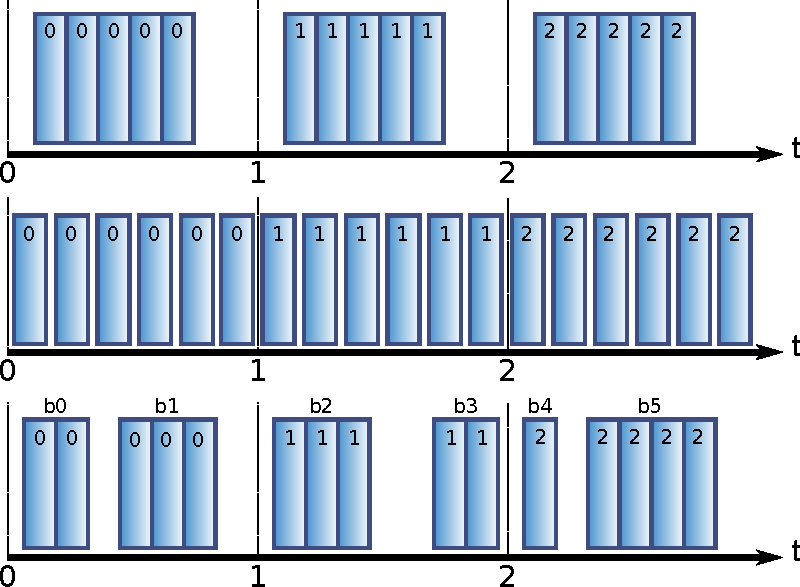
\includegraphics[trim=0mm 66mm 0mm 0mm, clip, width=0.6\textwidth]{rw-sgfd-modes2}
		\caption{Mode d'exécution à base temporelle}\label{fig:rw:sgfd:mode:time}
	\end{figure}
	\item Le mode basé sur les n-uplets au contraire considère que chaque n-uplet est une donnée à part entière. Le \textit{timestamp} n'est qu'une information du n-uplet pouvant être éventuellement utilisé par un opérateur de fenêtre, comme présenté sur la figure~\ref{fig:rw:sgfd:mode:tuple}.
	\begin{figure}[ht]
		\centering
		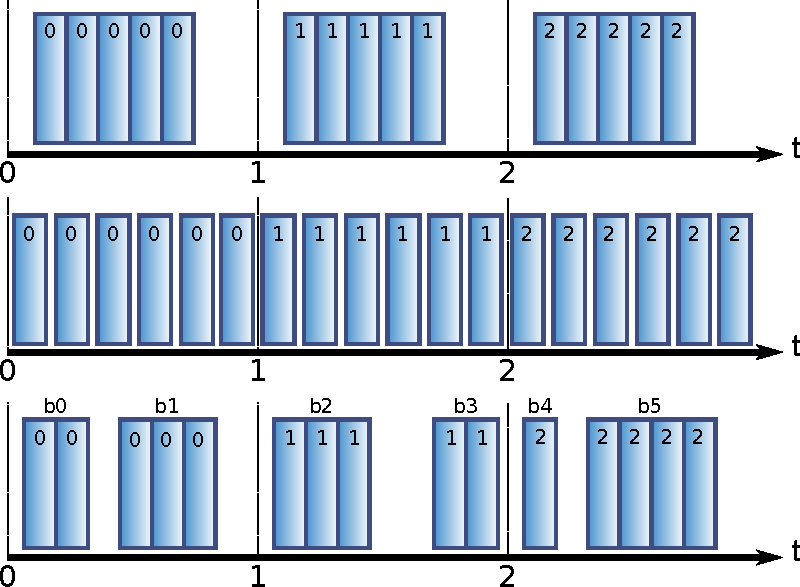
\includegraphics[trim=0mm 33mm 0mm 33mm, clip, width=0.6\textwidth]{rw-sgfd-modes2}
		\caption{Mode d'exécution basé n-uplet}\label{fig:rw:sgfd:mode:tuple}
	\end{figure}
\end{itemize}

Or, ces deux sémantiques rentrent effectivement en conflit sur certaines opérations, en voici un exemple :
\begin{example}\label{ex:rw:sgfd:batches}
 Soit $S$ un flux dont le contenu est, dans le formalisme \textit{ACO}, $\{\left<s_1,0\right>, \left<s_2,0\right>, \left<s_3,1\right>\}$. Nous souhaitons observer le résultat de la requête $S[1]$ (fenêtre de 1-tuple).

Si le modèle d'exécution est basé sur l'arrivée des n-uplets. Alors lorsque le n-uplet $s_1$ entre dans le système. Le système remplit une nouvelle fenêtre, ce qui donne $S[1](0)=\{s_1\}$. 

Le n-uplet $s_2$ est fournit et le système produit une nouvelle fenêtre : $S[1](0)=\{s_2\}$. Cette interprétation permet de considérer tous les n-uplets. Néanmoins, au même instant, la fenêtre a deux états différents, ce qui n'est pas correct d'un point de vue formel.

Si le modèle d'exécution est à base temporelle. Alors à l'instant 0, l'opérateur va obtenir les deux n-uplets. Puis, conformément à sa spécification algébrique, va sélectionner l'un d'eux, pour produire $S[1](0) = \{s_1\}$ ou $\{s_2\}$. Ceci est correct d'un point de vue formel, toutefois cet opérateur va perdre des données, ce qui peut être problématique.
\end{example}

Le problème est que les deux sémantiques ont du sens a priori. Pour clarifier, les auteurs introduisent la notion de \textit{batch}. Le \textit{batch} est une généralisation de ces modes puisqu'il considère que l'ensemble des n-uplets simultanés est partitionné en sous-ensembles ordonnés, comme représentés dans la figure~\ref{fig:rw:sgfd:mode:batch}. Ainsi, l'unité de temps d'exécution n'est pas le \textit{timestamp} ou l'n-uplet, c'est le \textit{batch}.
\begin{figure}[ht]
    \centering
		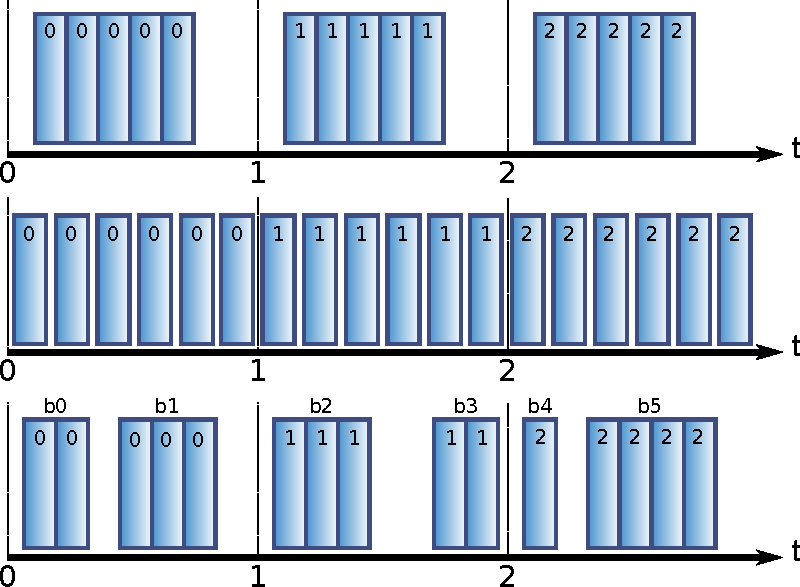
\includegraphics[trim=0mm 0mm 0mm 66mm, clip, width=0.6\textwidth]{rw-sgfd-modes2}
    \caption{Mode d'exécution basé \textit{batch}}\label{fig:rw:sgfd:mode:batch}
\end{figure}

Le \textit{batch} correspond à un envoi groupé de la part de la source. Deux événements peuvent se produire au même \textit{instant} (à l'unité de temps près)\footnote{Ces cas apparaissent facilement dans les cadres de grande échelle ou lorsqu'un événement est cause d'un autre, ou encore lors de la jointure d'un n-uplet avec plusieurs autres.}. Ainsi, lorsque la source effectue deux actions de production de données, ces actions correspondent à deux \textit{batchs} différents.

Des opérateurs sont développés pour manipuler les \textit{batchs} pour passer d'un mode d'exécution à l'autre. Par exemple, il est possible de structurer les \textit{batchs} d'un \textit{timestamp} donné à partir d'un autre attribut (identifiant par exemple).

De façon similaire, nous pouvons remarquer que dans l'algèbre \textit{ACO} la gestion de l'ordre positionnel est floue. Le flux est ordonné par \textit{timestamp}, mais en cas de n-uplets dits \textit{simultanés}, aucun ordre strict n'est définit. Dans la définition de la fenêtre positionnelle, \textit{ACO} introduit la définition d'une suite $(s_n)$ strictement ordonné. A. Arasu note sur ce point~\cite{Arasu:queries} : \enquote{\it Comme nous ordonnons arbitrairement la séquence $s_1$, $s_2$,..., les fenêtres positionnelles sont non déterministes lorsque les \textit{timestamps} ne sont pas uniques, ce qui peut ne pas être approprié}. L'introduction des \textit{batchs} apporte une généralisation de l'ordre temporel, ce qui permet de mieux maîtriser la sémantique d'exécution. Toutefois, s'il est nécessaire de faire un choix d'un nombre limité de n-uplets par exemple pour remplir une fenêtre, ce choix n'est pas spécifié.

Suite à l'identification des problèmes de modes d'exécution, le modèle \textit{SECRET}~\cite{Botan:secret} a été développé. Le principe est de décomposer l'opérateur de fenêtre en trois parties. Tout d'abord, le modèle décrit sa portée et son contenu (\textit{scope \& content}) pour savoir quels n-uplets sont inclus dans les fenêtres. Ensuite, les auteurs détaillent son mode de consommation de n-uplet (\textit{tick}), et enfin son mode de notification à l'utilisateur. Cette séparation claire des concepts permet d'avoir une meilleure compréhension des sémantiques possibles sur les fenêtres. Ainsi, ce modèle permet de décrire les modes de fonctionnement de systèmes existants pour mieux permettre leur intégration par la suite.

Les travaux de Krämer~\cite{Kramer:semantics} détaillent une algèbre de manipulation des flux. Le point novateur est la séparation des flux dits\textit{bruts}, \textit{logique} et \textit{physique}. 
\begin{itemize}
	\item Les flux tels que nous les avons décrit dans cette section sont des flux \textit{bruts} composés de couples $(\textrm{n-uplet},\textit{timestamp})$.
	\item Les flux logiques sont quant à eux un ensemble de triplets $(\textrm{n-uplet}, \textit{timestamp}, n)$. La multiplicité $n$ permet de compter le nombre d'occurrences du n-uplet a été observée dans le flux originel.
	\item Les flux physiques utilisent une définition très similaire à ce qui peut se trouver dans les bases de données temporelles avec un intervalle de validité. Ses éléments sont des couples $(\textrm{n-uplet},[t_s, t_e[)$.
\end{itemize} 
Deux algèbres sont ainsi décrites. La première manipule les flux logiques. Elle est utilisable pour correctement comprendre la sémantique des différents opérateurs. La seconde manipule les flux physiques qui sont utilisés par les implémentations des opérateurs. Des équivalences d'expressions sont ensuite définies pour passer du domaine logique au physique.

Enfin, les travaux sur SoCQ~\cite{Gripay:algebra} permettent d'exprimer une algèbre pouvant modéliser des extensions aux relations classiques de base de données. Ces extensions apportent des attributs pouvant être issus de flux ou des propriétés virtuelles fournies par des services logiciels\footnote{Au sens architecture à service du terme}. L'avantage d'une telle approche est de pouvoir intégrer rapidement les services issus de l'implémentation avec une gestion des données. Ainsi, nous avons une modélisation des sources mélangeant relations classiques et flux de données.

\section{Optimisations}
\TODO{ATTENTION CECI EST UN COPIER/COLLER DE NOTES DE PREMIÈRE ANNÉE}
\subsection{Optimisation dans les SGFD-R}
Le domaine de la gestion de flux de données a été largement influencé par la gestion de base de données. En effet, l'idée initiale était d'être capable de réutiliser les connaissances accumulées au cours des 40 dernières années dans ce domaine. Ainsi, afin de mieux analyser les optimisations de la gestion de flux, il devient important d'investiguer plus en détail le fonctionnement de la gestion de base de données.

\subsubsection{Le problème dans sa globalité}
Le processus d'optimisation usuel en gestion de base de données est maintenant établie et répendue~\cite{Ioannidis:optimization}. Une requête en gestion de base de donnée est soumise par un langage déclaratif tel que \textit{SQL}. A partir de cette expression, s'enchaine une série d'opération qui permettra l'exécution de celle-ci. La figure \ref{fig:rw:sgfd:optim:processus} décrit le processus complet nécessaire à l'aboutissement de ce traîtement. 
\begin{figure}[h]
\centering
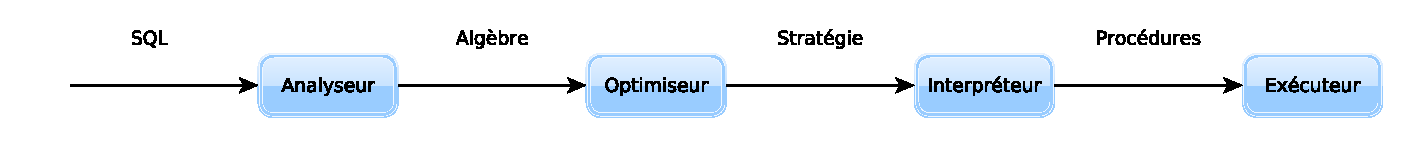
\includegraphics[width=0.9\textwidth]{rw-sgfd-optimsgbd}
\caption{Processus de traitement de requête dans un SGBD-R}\label{fig:rw:sgfd:optim:processus}
\end{figure}

Plusieurs modules permettent d'exécuter cette série d'opérations :
\begin{itemize}
    \item \textbf{Analyseur} : Prend en entrée une requête textuelle et fournit en sortie un arbre de requête écrit dans un format interne équivalent à de l'algèbre relationnelle. Ce module ne fait que traduire la grammaire du SQL par des règles prédéfinies.
    \item \textbf{Optimiseur} : Prend cet arbre de requête et fournit un autre arbre de requête, agrémenté d'indication de méthodes physique à utiliser. Le tout forme une stratégie d'exécution qui ne sera pas modifiée par la suite. Le but de cette étape est de fournir la stratégie qui fournit un résultat identique à ce que l'arbre initial était avec un coût moindre.
    \item \textbf{Interpréteur} : Récupère la stratégie d'exécution et instancie les procédures d'exécution. Le tout sera envoyé à l'\textbf{exécuteur} qui manipulera ces procédures afin de produire le résultat final.
\end{itemize}
L'optimiseur étant bien entendu le module le plus complexe car il possède et utilise beaucoup de connaissance et de résultats sur la gestion de données. Ce composant s'est prouvé indispensable dans la pratique car une bonne stratégie de traitement changera la plupart du temps de complexité ce qui transformera une requête pouvant être exécutée en plusieurs heures en moins d'une seconde.

Le problème est que l'espace des stratégies possibles pour exécuter une requête classique est potentiellement de cardinalité factorielle en fonction du nombre d'opérateurs et de méthodes d'exécutions disponibles (surtout s'il y a des jointures). Ainsi, il faut guider l'exploration et utiliser des techniques de programmation dynamique pour éliminer rapidement les branches trop coûteuses.

L'optimisation de requête se découpe en deux sections : l'optimisation logique (i.e. sélection du meilleur arbre d'opérateur théorique) et l'optimisation physique (choix des meilleurs algorithmes).

\subsubsection{Optimisation Logique}
L'espace algébrique est très large car les équivalences sur l'algèbre relationnelle sont très larges et permissives. Par exemple, une sélection sur une jointure $\sigma (R_1 \Join R_2)$ peut traverser l'opérateur binaire si sa condition ne concerne qu'une branche : $R_1 \Join \sigma R_2$. Ainsi, pour un arbre de requête, il peut y avoir des millions de requêtes équivalentes avec des permutations ou des ajouts d'opérateurs. Des heuristiques sont ainsi sélectionnées pour réduire cet espace tout en restant efficace~\cite{Ioannidis:optimization}. Le critère principal d'optimisation étant minimiser la taille des résultats intermédiaires. Voici les règles classiques :
\begin{itemize}
    \item[\textbf{R1}~:] \textit{La sélection et la projection n'introduisent pas de coût supplémentaires et sont traités à la volée}. Les sélections doivent être exécutés au moment de la première lecture sur la relation. Les projections doivent se faire en même temps que le résultat d'un autre opérateur.
    \item[\textbf{R2}~:] \textit{Les produits cartésiens ne doivent jamais être formés sauf si la requête elle-même en demande}. Seules les jointures peuvent combiner des relations.
    \item[\textbf{R3}~:] \textit{L'opérande interne (partie droite) de chaque jointure est une relation originelle, et non un résultat intermédiaire}.
\end{itemize}

La règle R1 est utilisée pour minimiser la taille des résultats intermédiaires. La règle R2 supprime toute possibilité de recours fatal aux algorithmes de boucles imbriquées sachant qu'un autre plan pouvait utiliser à chaque fois des jointures plus efficaces.

La règle R3 n'est pas toujours choisie car même si elle réduit beaucoup les possibilités car elle restreint les ordres de jointures, elle risque de supprimer l'arbre optimal dans plusieurs cas. En effet, les arbres de requêtes ne pourront pas être des arbres équilibrés car l'opérande droite doit être une relation native, or un arbre déséquilibré peut introduire des surcoûts du fait que les jointures supérieur doivent joindre une grande relation avec un résultat intermédiaire. Toutefois, il existe des raisons à cette règle. Tout d'abord, le fait d'avoir des relations natives permet l'utilisation d'index. De plus elle permet de faire un traitement total des requêtes en mode \textit{pipeline}\footnote{L'exécution en \textit{pipeline} permet de traiter un n-uplet dès sa lecture, notons que cela s'apparente à du traitement de flux. L'avantage étant que le processeur étant moins coûteux que les entrées-sorties, on peut rentabiliser l'attente de lecture en traitement de requête.}.

En parcourant l'espace algébrique des requêtes équivalentes vérifiant R1-3, le nombre de plans devient raisonnablement faible. Pour le reste des recherches, il sagit principalement de choisir l'ordre des jointures. Comme la jointure est symétrique $R_1 \Join R_2 = R_2 \Join R_1$ alors dans le cas de multiples jointures (courant en gestion de base de données), il faut choisir l'ordre le plus pertinent qui minimisera la taille des résultats intermédiaires. Cette recherche se fera conjointement avec l'optimisation physique du fait de son impact sur les algorithmes.

\subsubsection{Optimisation Physique}
L'optimisation physique correspond au parcours de l'espace des méthodes disponibles pour chaque plan de requête et à l'évaluation quantitative de chacune de celles-ci. L'espace des méthodes fournit plusieurs implémentation pour un opérateur. Par exemple pour la jointure :
\begin{itemize}
    \item \textbf{Boucles imbriqués} : Implémentation la plus directe de la jointure. Cet algorithme ne requiert aucune condition sur les relations d'entrées.
    \item \textbf{Jointure fusion} : Se base sur le fait que les deux relations sont triés sur l'attribut de jointure à l'avance. Ainsi la jointure est plus facile à effectuer. Elle est régulièrement utilisée avec des index triés comme les arbres B+~\cite{refneeded-b+tree}. Des opérateurs de tri pourront être déployés si ces index sont absent.
    \item \textbf{Jointure hachée} : Se base sur le fait que les deux relations sont hachées sur l'attribut de jointure. Ainsi la jointure se fait sur les index de hachages de cardinalité réduite et d'accès rapide.
\end{itemize}

Pour chaque relation, il existe deux moyens principaux d'accéder à un n-uplet :
\begin{itemize}
 \item \textbf{Scan} : Parcours strict de la relation ou d'un l'index pour trouver les n-uplets vérifiant une condition de sélection.
 \item \textbf{Probe} : Demande directement aux procédures d'index de renvoyer les tuples vérifiant une condition de sélection.
\end{itemize}

Ainsi, il est possible de faire des boucles imbriqués suffisamment performantes en utilisant des accès optimisés aux relations. Bien évidemment certaines sélections sont impossibles via les procédures d'index. Par exemple, il est impossible de demander à un index haché de faire une sélection avec un opérateur de comparaison tel que \enquote{$\leq$}.

L'évaluation de chacune de ces méthodes passe par un coût global de l'exécution basé sur des statistiques. Ces statistiques aideront à quantifier la taille des résultats intermédiaires. Pour cela, il est nécessaire de faire des calculs de sélectivité~\cite{Selinger:selectivity}. Ces calculs permettent d'évaluer le ratio d'n-uplet qui valident une sélection. Par exemple, en l'absence d'information complémentaire, une sélectivité de 10\% est appliquée par défaut. Par la suite chaque algorithme est capable de quantifier son coût en fonction de ces sélectivités et des cardinalités des entités manipulées.

Suivant les capacités du système et la taille de la requête, le système pourra réordonner les jointures pour optimiser les algorithmes. La recherche dans cet espace de méthode se base sur la programmation dynamique. Elle permet de faire une recherche exhaustive sans être extrêmement coûteuse (par des procédures de \textit{branch \& bound} usuelles).

\paragraph*{Optimisation de la recherche}
La recherche exhaustive peut être très coûteuse si les jointures sont nombreuses car l'espace des stratégies devient large, ce qui peut être long à calculer. Une approche heuristique est nécessaire pour avoir un temps de calcul qui permette un lancement rapide de la requête. 

Plusieurs approches existent, la plus connue reste basée sur la marche aléatoire sur le graphe des stratégies possibles. Celle-ci parcourt le graphe aléatoirement en reculant si le coût est devenu trop important. Une autre approche intéressante étant l'utilisation d'algorithmes génétiques pour résoudre ce problème. \textit{Postgres} utilise l'optimiseur \textit{Genetic Query Optimizer (GEQO)}~\cite{Postgres:geqo} si le nombre de jointure dépasse une certaine limite.

L'optimisation a été prouvée comme un problème NP-complet~\cite{Ibaraki:join} (même avec seulement les boucles imbriqués) ainsi certains efforts se sont concentré sur la résolution de sous cas importants, notamment boucles imbriqués et jointure hachée seulement.

\paragraph*{Base de données parallèles}
L'optimisation en prenant en compte des modèles de calculs parallèles est un problème encore ouvert. Toutefois, des approximations efficaces se basent sur les optimisations à deux phases. Tout d'abord, le système recherche la solution optimale comme vu précédemment. Par la suite, il cherche le meilleur ordonnancement. Les deux domaines ont été suffisamment couverts pour obtenir des résultats satisfaisants.

\paragraph*{Distribution du calcul}
La distribution du calcul est un problème différent des bases parallèles dans le sens où il existe plusieurs unités d'évaluation complètement indépendantes. Le problème toutefois se résout principalement en quantifiant la distribution du calcul à l'intérieur de l'espace des méthodes. L'espace de recherche sera toutefois plus grand et il faudra faire attention à avoir un optimiseur performant pour ne pas avoir de surcoût avant l'exécution.

\paragraph*{L'optimisation sémantique}
Supposons la présence d'une base de connaissance en parallèle de la base de donnée. Il est alors possible de raisonner sur les conditions de sélections notamment, afin d'amener plus ou moins de restriction à la requête. Les calculs d'inférence de concepts, comme vus en section~\ref{sec:rw:supervision:context}, permettent d'extraire des conditions plus restrictives mais équivalentes. Le problème étant d'avoir une base de connaissance suffisamment exploitable car une erreur de raisonnement pourrait supprimer potentiellement des résultats. De plus, les calculs d'inférences peuvent être lourds et ne doivent pas rendre le traitement de requête trop lourd. Cette approche commence a être exploitée en gestion de flux de données aussi grâce à des méta-données~\cite{Ding:semantic}.

\subsection{Optimisation spécifique de la gestion de flux}
\TODO{intro}
\subsubsection{Calcul incrémental}
Le principe fondateur de la gestion de flux étant que les données arrivent de manière continue. Comme présenté dans la section~\ref{sec:rw:sgfd:modeles}, les premiers traitement de flux~\cite{Terry:tapestry} étaient considérés comme des traitements particuliers sur des relations sans suppression ou mise à jour.

De façon plus générale, en se plaçant dans l'algèbre \textit{ACO} : Soit $R$ une relation, au lieu de calculer une requête sur $R(\tau)$, il est possible de considérer les \textit{delta} de cette relation : $\Delta_R^+(\tau) = R(\tau)-R(\tau-1)$ et $\Delta_R^-(\tau) = R(\tau-1)-R(\tau)$. Comme le traitement des fenêtres, par exemple, peut fournir directement ces différences : il n'y a donc pas de surcoût à l'utilisation d'un tel procédé. Comme la cardinalité des $\Delta$ est souvent minime face à celle de la relation totale. Il devient intéressant de travailler avec ces données.
\subsubsection{Load-shedding}
Contrairement aux approches classiques de gestion de base de données, il est important de voir que l'optimisation n'est pas toujours de pouvoir fournir les résultats exacts aux requêtes. L'objectif étant de fournir les résultats les plus pertinents possibles avec des contraintes d'espace mémoire, de temps de réponse ainsi que de charge réseau. En effet, comme la gestion de flux fonctionne de manière continue, une congestion dans le processus de traitement impliquera des retards et des complications pouvant aller jusqu'à une saturation du moteur.

L'idée du \textit{load-shedding} est de pouvoir abaisser ou limiter le taux de n-uplet au nombre suffisant pour pouvoir traiter sans introduire de retard. Dans les travaux fondateurs~\cite{Tatbul:window,Tatbul:load-shedding}, l'idée est de pouvoir surveiller le traitement des requêtes afin de reconnaitre les points d'engorgements et d'y implanter des opérateurs de shedding. Afin de garantir un certain taux de réussite, la politique qui sera utilisée pour le \textit{load-shedding} sera dirigée par une \textit{QoS}\footnote{QoS : Quality of Service} déterminant quelles données sont utiles. En effet, en prenant en entrée un graphe représentant \textit{valeur} $\mapsto$  \textit{taux de suppression acceptable}. Par exemple, dans le cadre d'une surveillance d'incendie, le taux de \textit{shedding} pour les températures inférieure à 20ºC pourra être très fort de part et d'autre du systèmes pour ce genre de données.


\subsubsection{Multi-Query Optimization (MQO)}
Aussi connu sous le nom de \textit{Global Query Optimization}. Cette optimisation profite des exécutions parrallèles pour éviter la redondances de traitement et une économie de ressources. Elle est issue du monde des SGBD~\cite{Sellis:mqo} et permet de répondre à plusieurs requêtes en même temps en utilisant des parties communes (classiquement, lorsque seules les clauses de sélection sont différentes). L'idée est toutefois peu exploitée car il faut pouvoir soumettre plusieurs requêtes en même temps et les gestions de caches ont permis de faire de bon résultat pour ce genre de requêtes. 

Dans le monde des flux de données, cette optimisation est largement reconnue comme importante. Les requêtes durant dans le temps, de façon potentiellement infinie, le nombre d'exécution concurrente sera donc très grand. Ainsi, partager les ressources des requêtes devient une façon d'optimiser grandement les requêtes. Plusieurs points interviennent ici.
\begin{itemize}
 \item Tout d'abord l'existence des \textit{m-op} (multi-operators)~\cite{Hong:mqo}. Ces opérateurs permettent de regrouper plusieurs opérateurs en un seul permettant d'éviter des duplicatas de n-uplets. Un exemple classique étant de grouper deux sélections sur un flux commun en une seule. Ainsi, si un n-uplet vérifie les deux sélections, un seul n-uplet sera fournit avec l'indication qu'il appartient aux requêtes 1 et 2. Cette optimisation permet de faire des requêtes en utilisant les définitions de flux fragmentés.
 \item Grande disponibilité des ressources. Chaque opérateur utilise des ressources et peut potentiellement les partager avec d'autres. Cependant, ces ressources ne sont peut-être pas utiles à partager car elles sont trop précises. Dans plusieurs travaux~\cite{Arasu:resource}, le calcul des agrégations sur fenêtres peut être partagé. En découpant la mémoire par bloc de façon intelligente, on peut partager les ressources afin d'économiser de la place mémoire.
\end{itemize}

Un problème ouvert reste de savoir si les optimisations locales (optimisation algébrique) gêneront les optimisations globales. Une requête ne possède pas qu'une seule optimisation au début de son traitement. En effet, si une nouvelle requête arrive et qu'en changeant légèrement la structure de la première, il est possible d'obtenir un partage, alors il est probable que ce nouveau plan soit le bon. L'adaptabilité d'une requête est donc importante.

\subsubsection{Ordonnancement}
Comme les requêtes s'exécutent en parallèle, la notion d'ordonnancement entre en compte. Afin d'éviter les engorgements, ou pour donner plus de priorité à une partie de la requête, l'ordonnanceur doit cadancer les unités de traitement pour fournir des résultats conformes à la qualité attendue. Par exemple, une requête importante (type alerte) peut exprimer des contraintes forte de \textit{latence}. A l'inverse, une requête d'observation passive aura des contraintes plus faible. Plusieurs stratégies ont été proposés~\cite{Babcock:chain, Jiang:scheduling} afin de garantir le meilleur temps de réponse en utilisant le moins de resources possibles.

\subsubsection{Routage}
Le problème du routage est un problème très connu du domaine des réseaux de capteurs où les contraintes de traitement sont si fortes au niveau de la transmission de données que les routages sont importants. Pour le traitement en flux de grandes quantités de données, des optimisations de routages rentrent en compte sur le calcul de jointure par exemple~\cite{Zhou:pmjoin}. En effet, il nous faut savoir s'il vaut mieux effectuer une opération lourde et ayant une sélectivité peut-être grande (>1) de façon distribuée avec transfert réseaux ou groupés mais plus chargés en traitement. 

De façon similaire, le coût (notamment énergétique) est analysé afin de fournir un routage au moment du placement de la requête~\cite{Galpin:snee} ou à l'exécution~\cite{Madden:tinydb}.

\subsection{Optimisation d'algorithmes}

\subsubsection{Jointures}
Comme présenté précédemment, la jointure en flux n'est pas aussi simple qu'une jointure au sens base de données car elle introduit la notion de fenêtre. Beaucoup de travaux~\cite{Han:join, Srivastava:join, Law:join} se sont portés sur les jointures similaires à $I_S (S_1[W_1] \Join ... \Join S_n[W_n])$ et bien souvent avec des fenêtres identiques. Car l'implementation de ceci requiert a priori une quantité non bornée de mémoire. De plus le traitement d'un n-uplet prendra du temps et il faudra pouvoir fournir le résultat sans retard par rapport aux flux d'entrées. 

Afin de garantir une exécution en temps réel, des procédés de load-shedding~\cite{Tatbul:load-shedding} sont mis en place en essayant de maximiser la pertinence des résultats, sortant ainsi du contexte de l'exécution exacte de requête. Le principe de base réside dans le fait de garder les n-uplets étant les plus pertinent. Ceci peut être basé sur le nombre de n-uplet que le n-uplet produira après calcul, ou celui qui est le plus agé. Le calcul de ceci peut se faire de façon différente :
\begin{itemize}
 \item Par un histogramme et un choix sur le nombre de tuple résultant~\cite{Han:join}
 \item Par un calcul probabiliste pour privilégier un flux plutôt qu'un autre pour sa productivité~\cite{Han:join}
 \item Par des raisonnements sur l'age du n-uplet~\cite{Srivastava:join}
\end{itemize}

L'utilisation d'index est désormais plus délicat car les données sont constamment actualisé. Le point crucial de l'index étant que le surcoût introduit au moment de l'insertion d'une donnée est amorti par le nombre de fois où la donnée sera interrogée. Il est toutefois important de noter que les optimisations présentes dans le calcul de jointures relationnelles en mode \textit{pipeline} sont ici applicables telles que le \textit{symmetric hash join}~\cite{Wilschut:symetricjoin} souvent appliqué.

D'autres optimisations ont été abordés sur la distribution du calcul~\cite{Zhou:pmjoin}. En effet, le coût engendré par les échanges fait que le calcul de la distribution des opérateurs devient importante. Dans cette optimisation, il est important de prendre en compte le partitionnement de la charge du flux par rapport au domaine des attributs de jointures. En effet, un attribut pourra avoir un débit très faible sur une valeur comparé à un autre qui sera bien plus présent. Des optimisations sur la distribution de ces calculs sont faisable.

Enfin, de façon un peu plus particulière, il est intéressant de noter les optimisations dans des contextes particuliers tels que le P2P (avec une DHT)~\cite{Palma:p2p}. Le calcul de la jointure peut se faire sur plusieurs noeuds afin de mieux distribuer le traitement.

\subsubsection{Fenêtrage et agrégations}
Nous nous intéressons maintenant particulièrement aux traitements de requêtes d'agrégations de classe $I_S(G(S[W]))$. Les travaux les plus conséquents se focalisent sur le fait de calculer de façon approximative des opérations de comptage et de quantile en mémoire limité~\cite{Arasu:window}. Ce comptage permet d'effectuer les autres statistiques en quantité restreinte~\cite{Datar:stats}, comme par exemple : 
\begin{itemize}
 \item Min/Max/Sum/Avg 
 \item Moyennes
 \item Tables de hachages
 \item Histogrammes
 \item Nombre de valeurs distinctes
\end{itemize}

L'approche est principalement mathématique et probabiliste. Par exemple, en se fixant une tolérance $\eps$, il est possible d'obtenir un résultat dans une quantité de mémoire prévisible.

\subsection{Synthèse}
Profitant des caractéristiques particulières en terme de contraintes de rapidité d'exécution, il y a eu de nombreux développement concernant l'optimisation dans les SGFD. Les plus gros efforts se sont concentrés sur le calcul d'algorithmes incrémentaux, ainsi que sur l'utilisation de réponses approximatives. Seulement quelques approches comme~\cite{Galpin:snee,Kramer:semantics} s'intéressent au fait de faire une optimisation de plan de requête (logique puis physique). Toutefois, le manque de connaissance dans le domaine théorique de la gestion de flux de données fait que les équivalences de requêtes sont peu nombreuses en dehors des usuelles~\cite{Slivinskas:temporal,Arasu:stream}.

Ainsi, comparé à l'optimisation des SGBD, seules les règles évidentes telles que l'application de projections au plus près des sources sont faites dans l'optimisation logique. Peu de parcours de plans de requêtes et de stratégies d'exécutions équivalentes n'est appliqué. De même, la prise en considération des autres requêtes pour le partage de résultat intermédiaire est une stratégie efficace. Toutefois, cette opération est principalement faite de façon manuelle à l'installation d'une nouvelle requête. Seul des travaux comme RUMOR~\cite{Hong:mqo} recherchent à fusionner le nouveau plan de requête avec un autre (sous condition strictes).

Nous pouvons donc conclure que l'optimisation en gestion de flux de données a été grandement recherchée et a produit de multiples techniques. Toutefois, une utilisation de ces techniques pour faire une \textbf{recherche d'optimisation globale} sans intervention de l'utilisateur est encore limitée notamment du au manque de connaissance théorique.



%
%\subsubsection{Désignation}
%La désignation est une opération coûteuse car elle nécessite de parcourir a priori l'ensemble du réseau pour savoir si telle ou telle source vérifie les conditions que l'on a posé. Des structures d'index ont étés ainsi mises en place notamment dans les réseaux de capteurs~\cite{Greenstein:difs}. Principalement, le but reste de pouvoir faire des recherches de device sur des données de haut niveau sémantique. Par exemple, il peut être utile de savoir qu'un groupe de capteur possède une température entre 20 et 30ºC. Ce qui fait que lors de la recherche d'un capteur émettant entre 20 et 25ºC, il suffira d'affiner la recherche dans ce groupe ci. 
%
%Des recherches probabilistes se sont penchés dessus~\cite{Bhattacharya:mist}, en permettant de prédire le comportement d'une donnée au fur et à mesure du temps avec des chaines de Markov. Cette structure de données fournit un très bon contexte de désignation <<rapide>>.
%
%Bien évidemment, toutes les recherches sur les infrastructures distribués permettent de répondre en terme d'optimisation. Par exemple, que ce soit des infrastructures de gestion de données de devices directement~\cite{Gurgen:sstreamware}, ou tout simplement dans le contexte P2P, l'utilisation de DHT.
%
%\subsubsection{Historique}
%Le stockage historique est une partie peu abordée dans le monde des flux de données car celle-ci passe directement dans le monde des bases de données qui sont connues maintenant. Toutefois le contexte des flux de données fait que d'autres optimisations peuvent être opérées. Un des travaux fondateurs serait~\cite{Chandrasekaran:oscar} qui avance le fait que les structures d'index habituelles (arbres B+) ne sont pas optimales dans ce contexte. En effet, l'index portant sur le \textit{timestamp}, et l'insertion se faisant presque toujours dans l'ordre croissant il est facile de trouver une structure plus adaptée. Comme beaucoup de travaux, celui-ci apporte le fait de pouvoir s'adapter à la charge en supprimant certains n-uplets à l'avance.
%
%Pour ne pas perdre de données, il faut ainsi se tourner vers le domaine des \textit{data-warehouses}~\cite{Chaudhuri:warehouse} afin d'avoir de bonnes performances à l'insertion. Seulement, leur modèle de donnée fait que les requêtes auront du mal à être optimisés pour un résultat rapide. Des approches plus consensuelle~\cite{Petit:historical} ont étés mises en place pour s'adapter à la charge (en jouant sur le retard à l'insertion) sans perdre de données. Bien sûr, on introduit ainsi une limite de traitement. 
%
%Enfin, un dernier mode de stockage sont les informations résumés~\cite{Diao:stonedb}. En effet, en considérant que l'on stocke à l'intérieur de la base de données des moyennes ou des images en moindre résolutions (pour les caméras), on peut gagner énormément en performances sans grandement détruire la sémantique du stockage. Certains travaux~\cite{Diao:stonedb} proposent de stocker au plus proche des appareils les données détaillés et d'utiliser les passerelles réseaux comme cache avec des données résumés. Les résumés peuvent être issus de la communauté du data mining. 
